\chapter{Descriptive statistics}
\label{app:descriptives}

\FloatBarrier
\section{Gender}

\begin{longtable}[c]{@{}lrrrr@{}}
\toprule\addlinespace
& Total & Male & Female & Other
\\\addlinespace
\midrule\endhead
\textbf{Flashcards} & 12 & 7 & 5 & 0
\\\addlinespace
\textbf{Flashmap} & 11 & 8 & 3 & 0
\\\addlinespace
\textbf{Total} & 23 & 15 & 8 & 0
\\\addlinespace
\bottomrule
    \label{tab:gender}
\end{longtable}

\FloatBarrier
\section{Age}

\begin{longtable}[c]{@{}lrrrrrrrrrr@{}}
\toprule\addlinespace
& N & min & max & mean & var & skew & kurt & normal-t & normal-p
\\\addlinespace
\midrule\endhead
\textbf{Flashcards} & 12 & 15 & 17 & 15.75 & 0.39 & 0.15 & -0.52 & 0.096
& 0.9530
\\\addlinespace
\textbf{Flashmap} & 11 & 15 & 17 & 15.73 & 0.42 & 0.25 & -0.62 & 0.211 &
0.8997
\\\addlinespace
\textbf{General} & 23 & 15 & 17 & 15.74 & 0.38 & 0.20 & -0.57 & 0.307 &
0.8576
\\\addlinespace
\bottomrule
    \label{tab:age}
\end{longtable}

\begin{figure}[htbp]
    \centering
    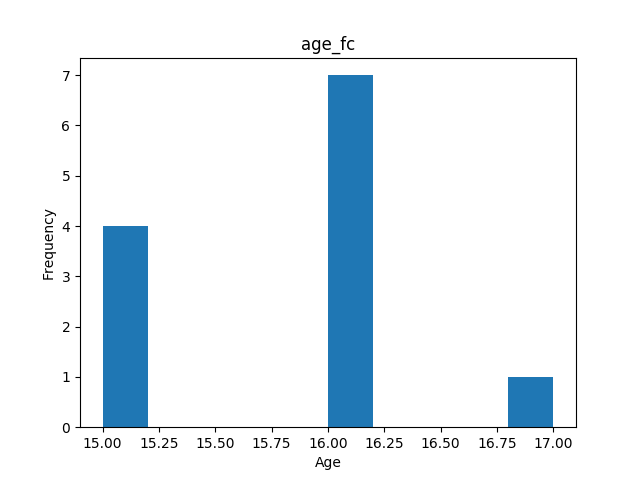
\includegraphics{img/age_fc.png}
    \caption{A histogram of the age of the flashcard users finishing the experiment}
\end{figure}
\begin{figure}[htbp]
    \centering
    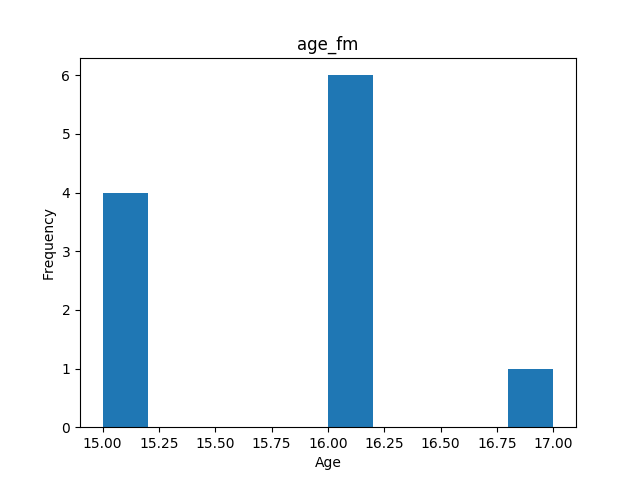
\includegraphics{img/age_fm.png}
    \caption{A histogram of the age of the flashmap users finishing the experiment}
\end{figure}
\begin{figure}[htbp]
    \centering
    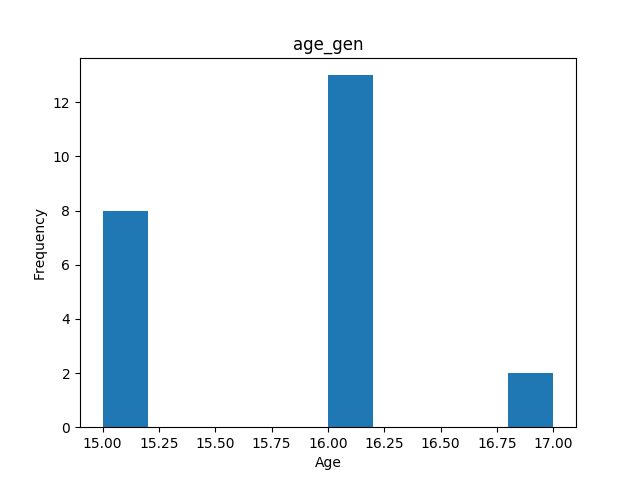
\includegraphics{img/age_gen.png}
    \caption{A histogram of the age of all users finishing the experiment}
\end{figure}

\FloatBarrier
\section{Comparisons of ages among conditions}

\FloatBarrier
\subsubsection{Age}

\begin{longtable}[c]{@{}lrrrr@{}}
\toprule\addlinespace
& \textbf{Mann-Whitney-U k} & \textbf{Mann-Whitney-U p} &
\textbf{Welch's t-test k} & \textbf{Welch's t-test p}
\\\addlinespace
\midrule\endhead
& 0.086 & 0.9323 & 0.086 & 0.9325
\\\addlinespace
\bottomrule
    \label{tab:age_comp}
\end{longtable}

\begin{figure}[htbp]
    \centering
    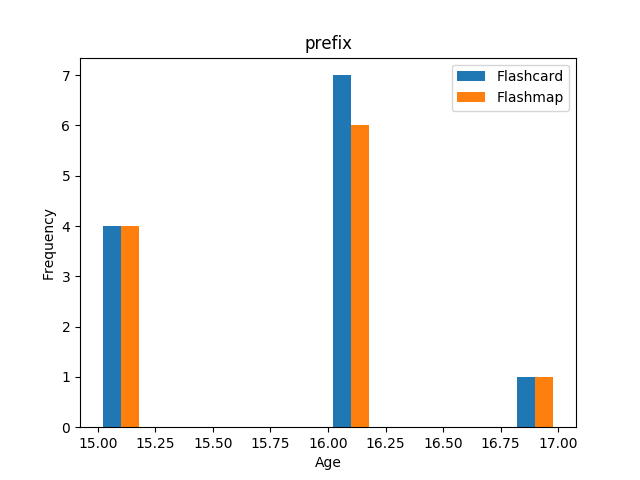
\includegraphics{img/age.png}
    \caption{Age comparisons of flashcard and flashmap users}
\end{figure}
